%%%%%%%% this is our results and comparison

%\documentclass[12pt, amstex, letterpaper] {report} %{article}


\usepackage[margin=1in]{geometry}
\topmargin -0.5in \textwidth 6.5in \textheight 9in
\footskip .5in
\headheight 0.3in


\usepackage{Sweave}

\DefineVerbatimEnvironment{Sinput}{Verbatim} {xleftmargin=0em,frame=single}
\DefineVerbatimEnvironment{Soutput}{Verbatim} {xleftmargin=0em,frame=single}

\usepackage{amssymb, mathrsfs, amsmath, amsfonts}
\usepackage{enumerate, comment}
\usepackage{hyperref, natbib,apalike, float} %cite
\usepackage{color, multirow, setspace, fancyhdr,graphicx}
\usepackage{undertilde}
\usepackage[bottom]{footmisc}
\usepackage{graphicx}
\usepackage{framed}
\usepackage{subcaption}
\usepackage{amsthm}

%\doublespacing
\pagestyle{empty}
\pagestyle{fancy}
\lhead{ }
%\rhead{May 2016}
\fancyfoot{ }
\rfoot{Dissertation $|$ \thepage}
\lfoot{Chris Vanlangenberg}
\date{}

\includecomment{comment}

\newtheorem{theorem}{Theorem}[section]
\newtheorem{defn}{Definition}[section]
\newtheorem{prop}{Proposition}
\newcommand{\pro}[1]{\begin{prop}{#1}\end{prop}}

%\newtheorem{proof}{proof}
\newtheorem{rmk}{Remark}
\newcommand{\rmark}[1]{\begin{rmk}{#1}\end{rmk}}

\numberwithin{equation}{section}
\renewcommand{\footrulewidth}{0.1pt}
\renewcommand{\headrulewidth}{0.1pt}


\newcommand{\eqn}[1]{\begin{equation}{#1}\end{equation}}

\newcommand{\beq}{\begin{equation}}
\newcommand{\eeq}{\end{equation}}
%\renewcommand\refname{Literature}
\newcommand{\blue}[1]{\textcolor{blue}{\emph{#1}}}
\newcommand{\red}[1]{\textcolor{red}{\emph{#1}}}
\newcommand{\twoc}[2]{{\textcolor{blue}{#1}} and {\textcolor{red}{#2}}}


\newcommand{\xn}{x_1,\ldots, x_n}
\newcommand{\Xn}{X_1,\ldots, X_n}
\newcommand\floor[1]{\lfloor{#1}\rfloor}
\newcommand\ceil[1]{\lceil{#1}\rceil}

\newcommand{\X}{\mathcal{X}}
\newcommand{\Sp}{\mathbb{S}}
\newcommand{\R}{\mathbb{R}}
\newcommand{\C}{\mathbb{C}}
\newcommand{\pd}{positive definite }



\newcommand{\code}[1]{{\small\texttt{#1}}}
\newcommand{\pkg}[1]{{\normalfont\textsf{#1}}}
\newcommand{\var}[1] {{\normalfont\textbf{#1}}}
\newcommand{\Cm}{$C_m(\phi_P, \phi_Q)\ $}

\newcommand{\jun}{\cite{JunStein2008}}
%\begin{document}

Currently to our knowledge currently there are no methods developed totest axially symmetry in  global data. Therefore, to validate the compatibility of generated axially symmetry global data we compared the MOM estimates to its theoretical values. It is somewhat difficult to model the covariance structure in other terms to generate data when it is closer to Earth's pole (the complexity can be observed in MSU and TOMS data). Therefore, to demonstrate some snapshots of the generated the latitudes were trimmed above $60^0$N and below $60^0$S yet we provide a very high resolution $120\times 180\ (n_l\times n_L)$ for simulate data. The parameters were fixed, $C_1 = 1, C_2 = 1, a = 1, u = 1$ and $p=0.5$, to generate data on a sphere. In the proposed model 1 $c_0 = C_0(\phi_P, \phi_Q)$ which provides a non zero mean random process on a sphere, if the process is non-zero mean we showed that (in chapter 4) cross covariance is biased with a bias of $c_0$. However,  model 2 and 3 yields a zero mean process on a sphere. Regardless of the mean the cross variogram is unbiased. Four snapshots of the gridded data generated based on model 2 is given below (refer appendix A \ref{appendixA} for data snapshots on other models). 

\begin{figure}[H]
	\label{grid_plot_model2}
	\begin{center}
		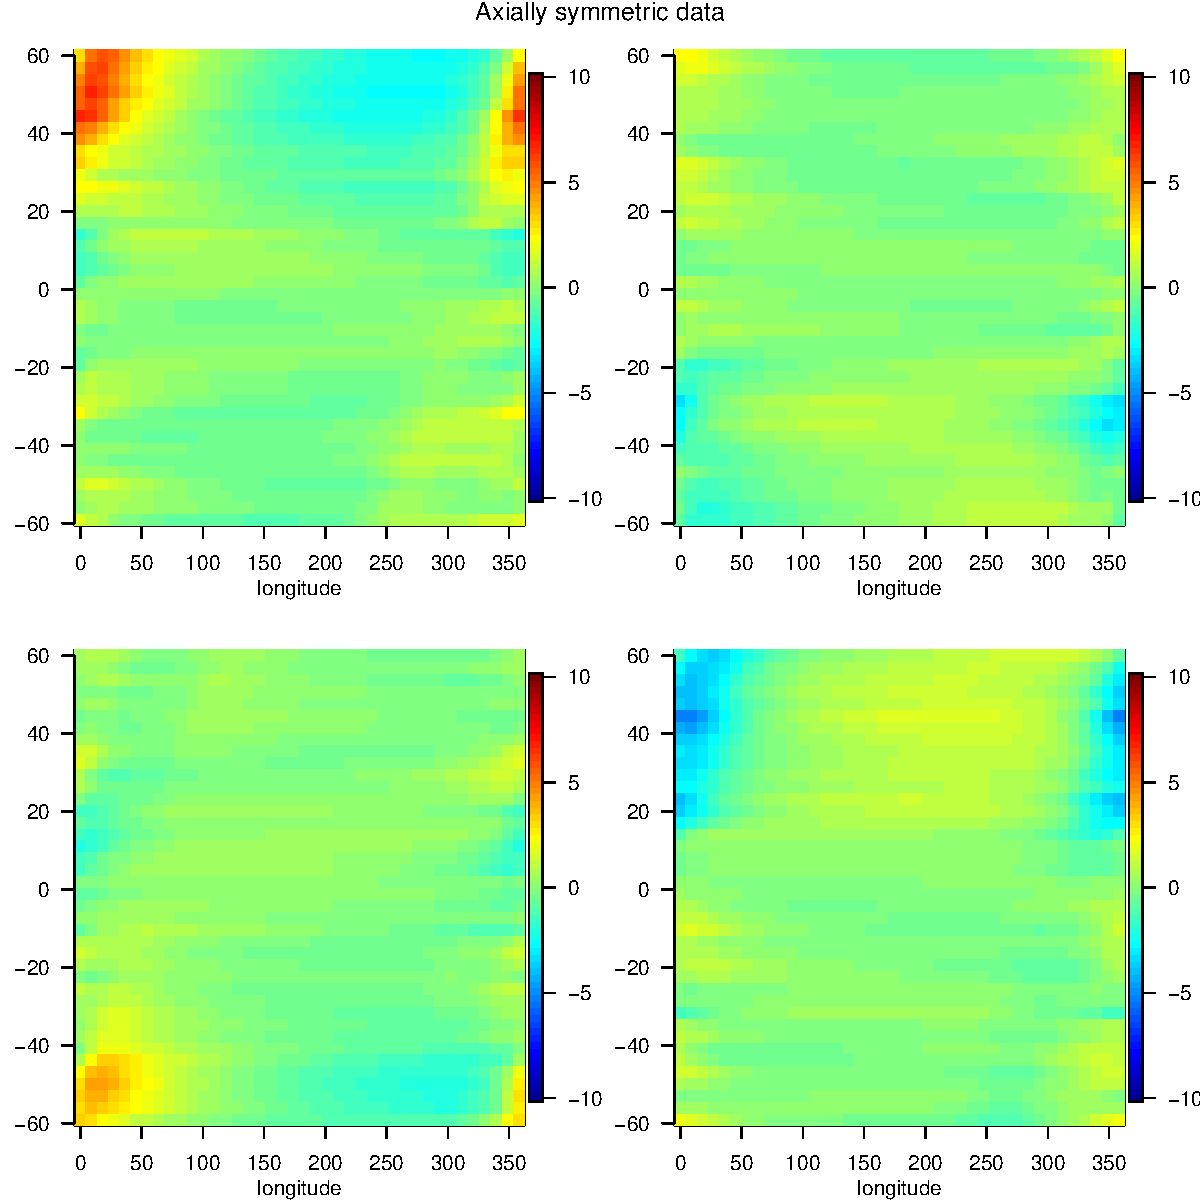
\includegraphics [width=0.9\textwidth ]{graphs/Data_sample_120_model2.pdf}
		\caption{Four consecutive axially symmetric data snapshots based on model 2, grid resolution $2^0\times 1^0$ (data scale -10 and 10).}
	\end{center}
\end{figure}

The above snapshots are some what compliance with geo-spatial data (MSU and TOMS), clearly there is a spatial trend within each latitude but not within longitudes. We observed some inconsistencies (strong spots) closer to the boundary points of longitudes ($\lambda \rightarrow 0,\lambda \rightarrow 2\pi$) and we have ignored the tilt (approximately $23^0$) of Earth axis, both of these are left out as future studies. The figure \ref{grid_plot_model2_sim2} refers to the second snapshot (top right) of the generated data and it is clearly evident that trends are within latitudes.     

\begin{figure}[H]
	\label{grid_plot_model2_sim2}
	\begin{center}
		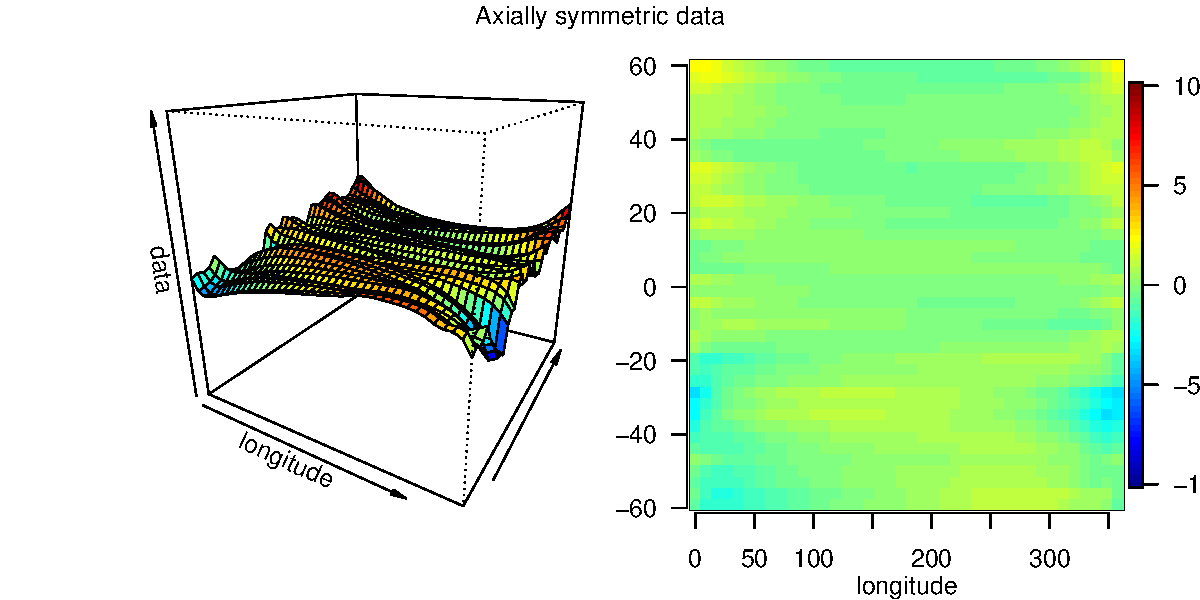
\includegraphics [width=0.9\textwidth ]{graphs/Data_sample_120_model2_density.pdf}
		\caption{One snapshot of the axially symmetric data generated based on model 2, grid resolution $2^0\times 1^0$ (data scale -10 and 10)Data distribution over the grid.}
	\end{center}
\end{figure}

%-------------------------------------% 
\subsection{Comparison of the proposed models with MOM estimates}
%-------------------------------------%

We consider two latitudes with larger latitude difference in order to capture the largest possible errors $70^0S$ and $60^0N$ ($\phi = 10, 150$) with 100 longitudes and compared the MOM estimators.

\begin{figure}[H]
	\begin{subfigure}{.5\textwidth}
		\centering
		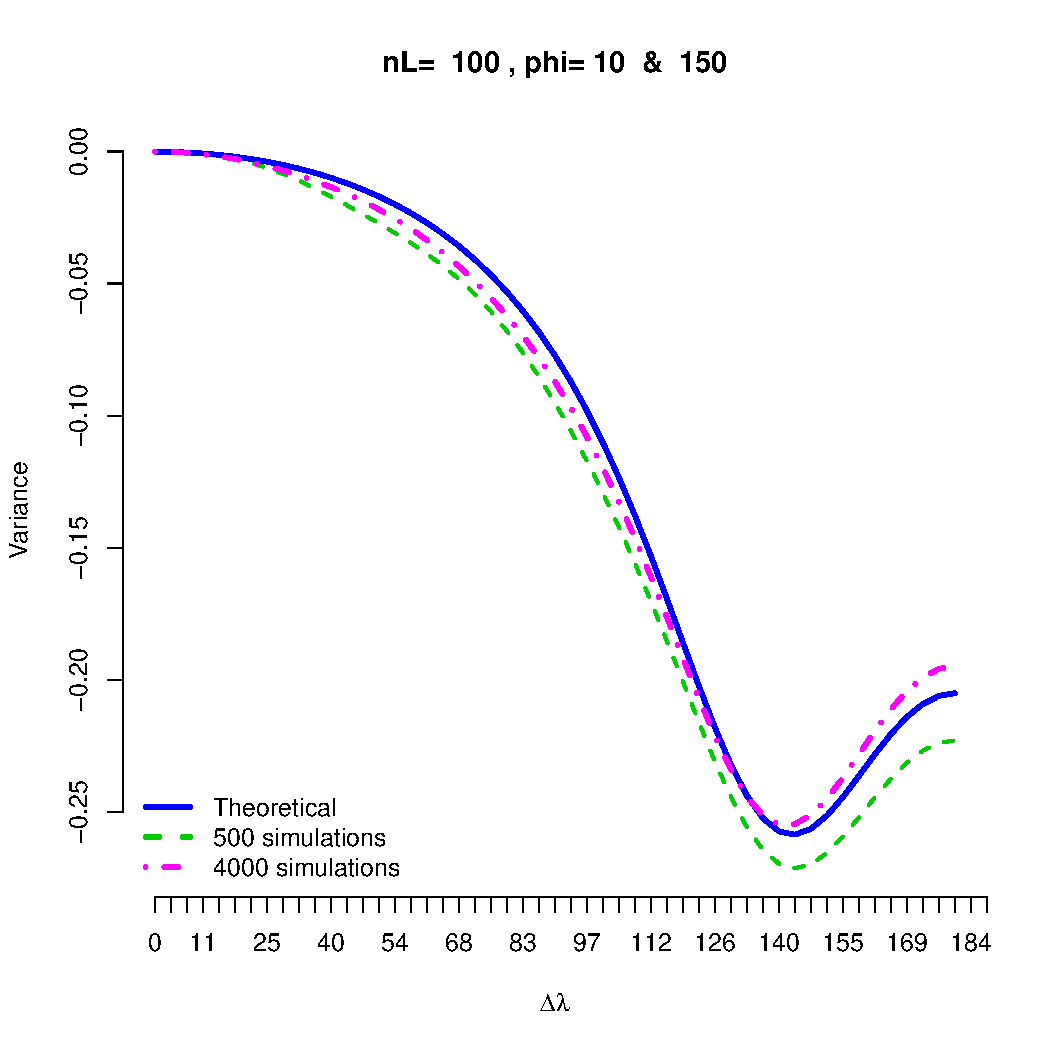
\includegraphics[width=1\linewidth]{graphs/results_variogram_model1}
		\caption{parameter set 1}
		\label{fig:sfig1}
	\end{subfigure}
	\begin{subfigure}{.5\textwidth}
		\centering
		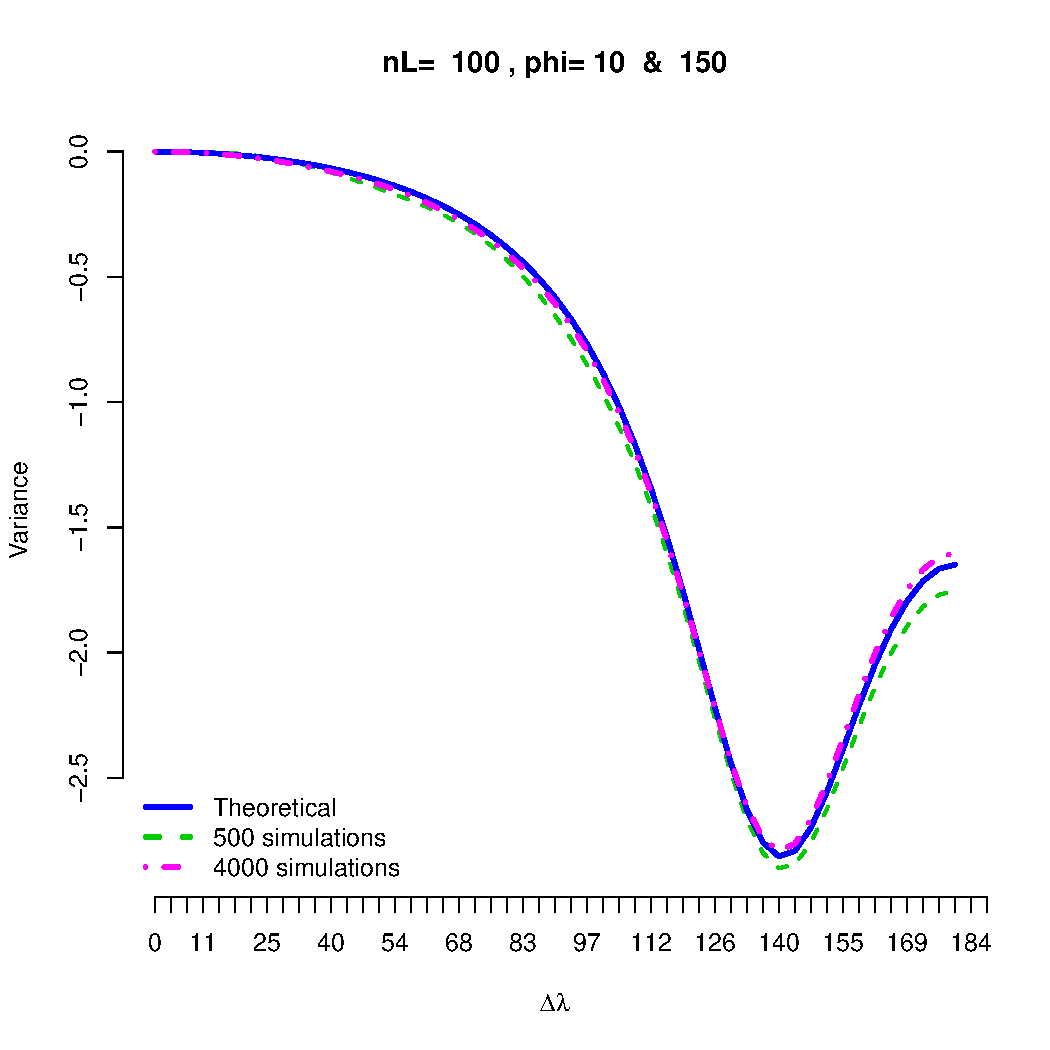
\includegraphics[width=1\linewidth]{graphs/results_variogram_model1_2}
		\caption{parameter set 2}
		\label{fig:sfig2}
	\end{subfigure}
	\caption[Cross variogram estimator comparison]{Cross variogram estimator comparison for covariance model1 }
	\label{compare_varigram_sim}
\end{figure}

The cross variogram estimator (\ref{cross_variogram}) is unbiased and in case of circle we showed that the variogram estimator is inconsistent and we expect a similar result in the case of sphere (the proof is left out as future work). Since model 1 is a non zero mean process we use the cross variogram estimator () to compare the generated data. We used two different sets of parameters to compare the cross variogram for model 1, set 1 $C_1 = 1, C_2 = 1, a = 1, u = 1$ and $p=0.5$ and set 2 $C_1 = C_2 = 2, a = =3, u = 1$ and $p=0.6$. The rate of convergence (\blue{should we talk about any theoretical properties of convergence since we don't have a proof for consistency}) is very slow as one can see that when number of simulations were increased from 500 to 4000 the cross variogram estimator is much closer to its theoretical value. However, the cross variogram estimator for model 2 and 3 converges much faster compared to model 1.  

%-------------------------------------% 
\subsubsection{Results for longitudinally reversible processes}
%-------------------------------------%

The parameter $u = 0$ yields a longitudinally reversible processes on a sphere (see Figure \ref{fig_parameter_comp} 1(d) ) regardless of the model. Now the cross variogram estimator converges ({\em a.s.}) to its theoretical value much faster (< 500 simulations).          

\begin{figure}[H]
	\centering
	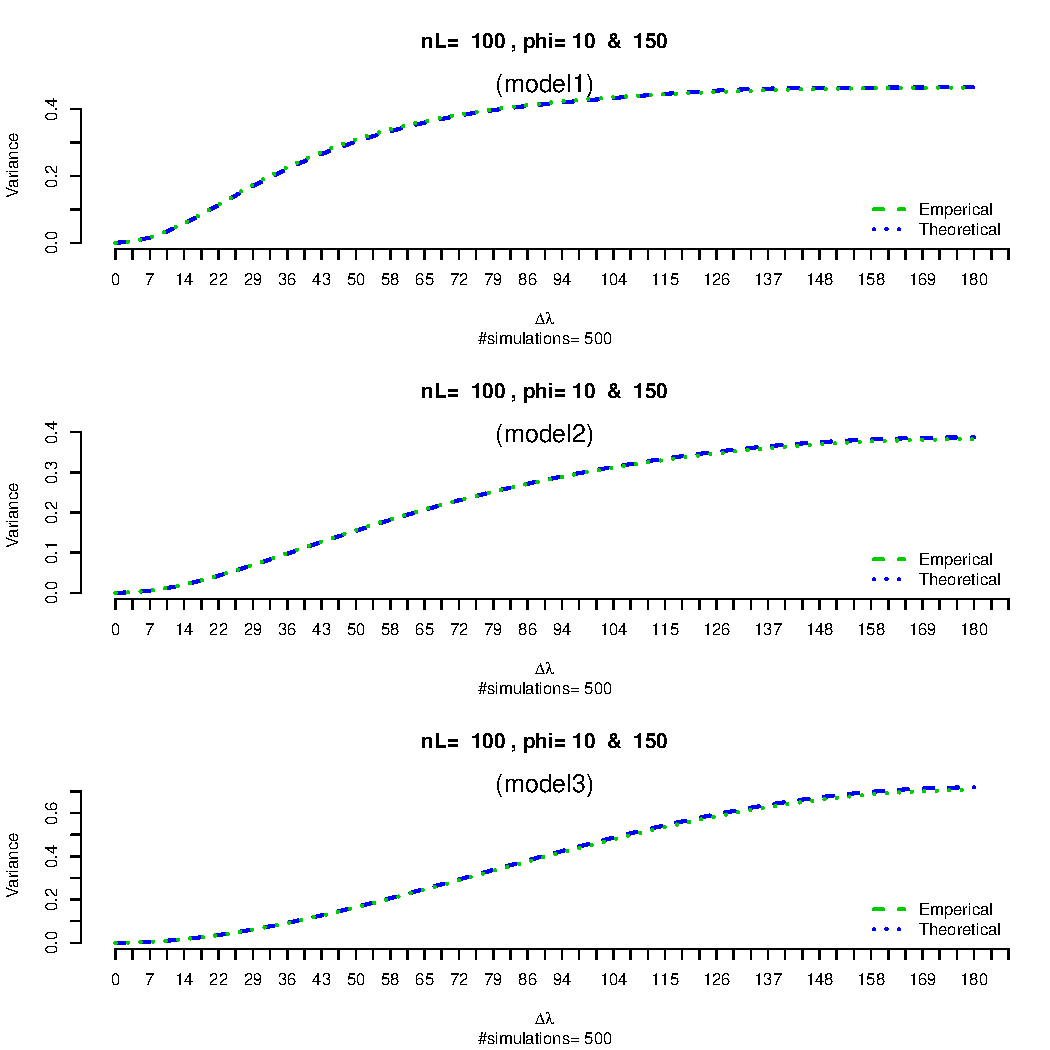
\includegraphics [width=0.9\textwidth ]{graphs/results_variogram_comparison}
	% width=12cm,height=12cm
	\caption[Variogram comparison]{Cross variogram estimator comparison over model 1, model 2, model 3 when $u=0$ }
\end{figure}

Next, we compared the cross covariance estimator on zero mean processes (model 2, model 3) on a sphere. In order to compare the cross covariance we used two pairs of latitudes $20^0S$ with $10^0S$ ($\phi = 70, 80$) and $30^0S$ with $40^0N$ ($\phi = 60, 120$). In a zero mean process, the rate of convergence depends on the distance between the latitudes.    

% \begin{figure}[H]
% \begin{center}
% 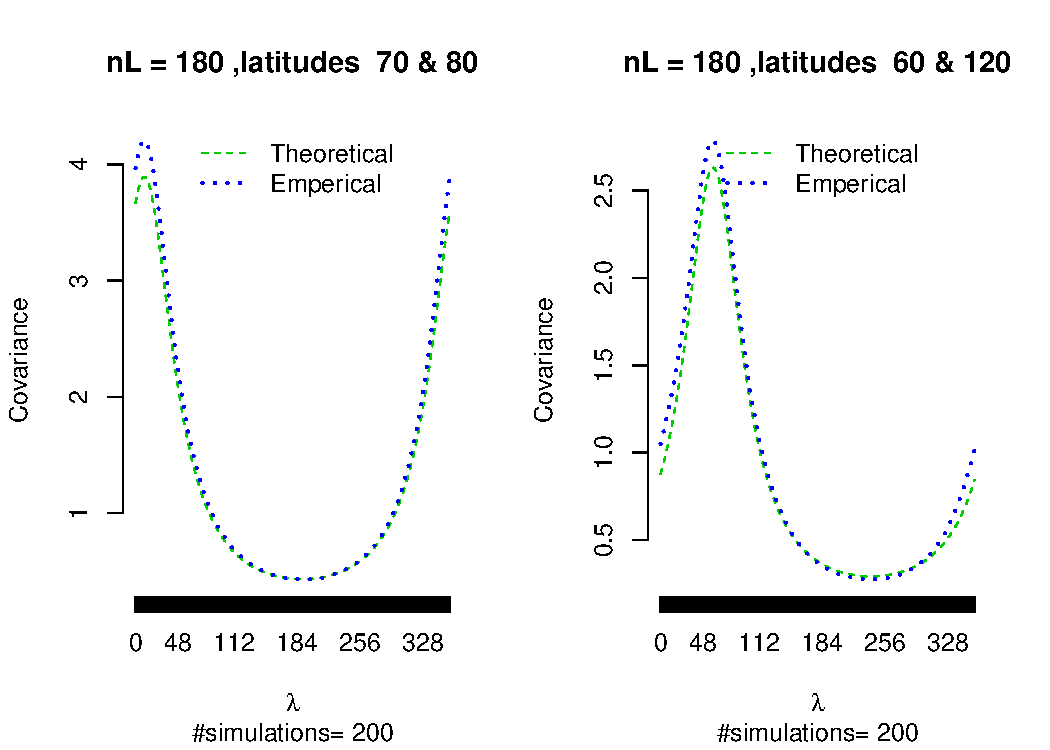
\includegraphics [width=0.75\textwidth ]{graphs/Model1.pdf}
% \caption{Cross covariance comparison of model1}
% \end{center}
% \end{figure}



\begin{figure}[H]
	\begin{center}
		\includegraphics [width=0.75\textwidth ]{graphs/Model2.pdf}
		%\includegraphics [width=6in, height=3in]{Model2.pdf}
		\caption{Cross covariance comparison of model 2}
	\end{center}
\end{figure}


\begin{figure}[H]
	\begin{center}
		%\includegraphics [scale=.6]{Model3.pdf}
		\includegraphics [width=0.75\textwidth ]{graphs/Model3.pdf}
		\caption{Cross covariance comparison of model 3}
	\end{center}
\end{figure}




%\end{document}
